\documentclass[a4paper,12pt]{scrartcl}
\usepackage[utf8]{inputenc}
\usepackage[UKenglish]{isodate}
\usepackage{csquotes}
\usepackage{graphicx}
\usepackage{wrapfig}
\usepackage{enumitem}
\usepackage{pdflscape}
\usepackage[toc,page]{appendix}
\usepackage{geometry}
\usepackage{hyperref}
\usepackage{cleveref}
\usepackage{listings}
\usepackage{csvsimple}
\usepackage{booktabs}
\usepackage{longtable}
\usepackage{caption}
\usepackage{subcaption}
\usepackage[colorinlistoftodos]{todonotes}
\usepackage[british]{babel}
\usepackage{float}
%\usepackage[margin=1in]{geometry}
\usepackage{listings}
\usepackage{color}
 
\definecolor{codegreen}{rgb}{0,0.6,0}
\definecolor{codegray}{rgb}{0.5,0.5,0.5}
\definecolor{codepurple}{rgb}{0.58,0,0.82}
\definecolor{backcolour}{rgb}{0.95,0.95,0.92}
 
\lstdefinestyle{mystyle}{
	language=PHP,
    backgroundcolor=\color{backcolour},   
    commentstyle=\color{codegray},
    keywordstyle=\color{magenta},
    numberstyle=\tiny\color{codegray},
    stringstyle=\color{codegreen},
    basicstyle=\footnotesize,
    breakatwhitespace=false,         
    breaklines=true,                 
    captionpos=b,                    
    keepspaces=true,                 
    numbers=left,                    
    numbersep=5pt,                  
    showspaces=false,                
    showstringspaces=false,
    showtabs=false,                  
    tabsize=3,
    morekeywords={ new, __halt_compiler, abstract, and, array, as, break, callable, case, catch, class, clone, const, continue, declare, default, die, do, echo, else, elseif, empty, enddeclare, endfor, endforeach, endif, endswitch, endwhile, eval, exit, extends, final, for, foreach, function, global, goto, if, implements, include, include_once, instanceof, insteadof, interface, isset, list, namespace, new, or, print, private, protected, public, require, require_once, return, static, switch, throw, trait, try, unset, use, var, while, xor}
}

\lstset{language=Java,
  showspaces=false,
  showtabs=false,
  breaklines=true,
  showstringspaces=false,
  breakatwhitespace=true,
  commentstyle=\color{pgreen},
  keywordstyle=\color{pblue},
  stringstyle=\color{pred},
  basicstyle=\ttfamily,
  moredelim=[il][\textcolor{pgrey}]{$$},
  moredelim=[is][\textcolor{pgrey}]{\%\%}{\%\%}
}
 
\lstset{style=mystyle}

\graphicspath{ {images/} }
\usepackage[
	backend=biber,
	style=ieee,
	]{biblatex}

\addbibresource{references.bib}

\title{Case study of A National Programme for IT with regards to Managing Software Intensive Projects}
\author{James Fernando}
\date{\today}

\begin{document}
	
	\begin{titlepage}
		\maketitle
	\end{titlepage}
	
	\tableofcontents
	\newpage
	\section{Introduction}
	{
		This case study will initially take you through the background of the National Programme for IT (sometimes referred to as NPfIT) before then going on to look at various project management details of the project. This includes the project goals, the type of project and a NTCP diamond for the project, is the project a Copps project, the project lifecycle and phases of the project, how the user/stakeholders of the project were consulted before and during the project, the software engineering methods used and their suitability to the project, the project organisation and if/how this could have been better implemented, integration with current systems and how the transfer of data will take place, before finally concluding on the project its successes and failures and a brief recap of the points made in the report.
	}
	\section{Project Background}
	{
		NHS Connection for health is a section of the Department of Health which was in charge of producing a national programme for IT to allow for the sharing of patient information, this was set up in 2005\cite{nhsconnectingforhealth2019}. However some of the ideas for centralising patient information had been published in 1998. The quote below lists a couple of the ideas listed in a book published by the Department for Health in 1998.
		\begin{displaycquote}{frankburns1998}
			\label{qoute:ConnectingForHealthPlans}
			individualised personal electronic records will be developed to provide NHS
			professionals with 24 hour secure access to the information important to
			individual patients’ care, when required. This will immeasurably improve
			emergency care and ensure any professional involved in the care of an
			individual is up to date with their treatment
			
			on-line services will be provided for GPs and their patients, to make hospital
			appointments as required or diagnostic results when due. The sight of hard
			pressed NHS professionals rummaging about in buff folders or hand-writing
			referrals and test requests will be consigned to history as soon as possible.
		\end{displaycquote}
		
		\begin{figure}
			\centering
			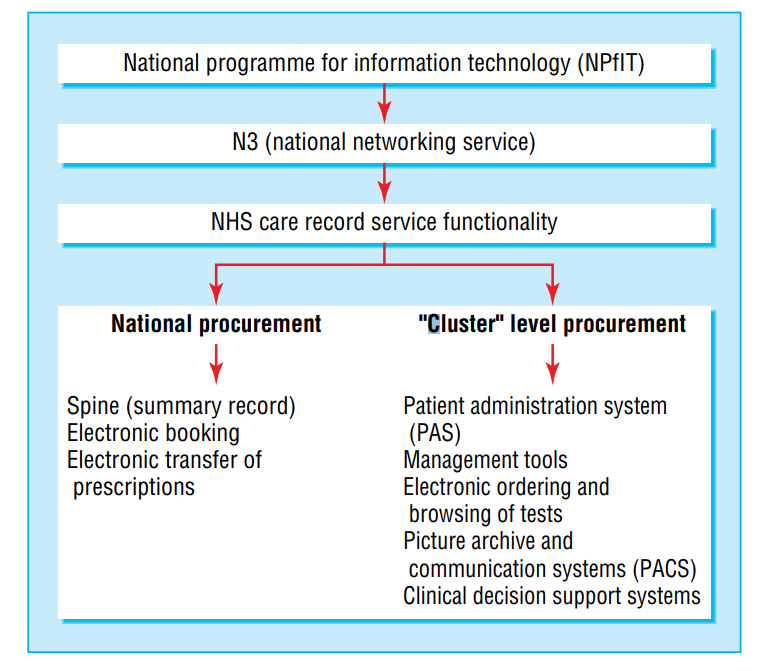
\includegraphics[width=\textwidth]{NPfITServicesOutline}
			\caption{Shows a break down of the services and systems which make up the National Programme for IT\cite{Hendy2005}}
			\label{fig:NPfITServicesOutline}
		\end{figure}
		\Cref{fig:NPfITServicesOutline} shows how the project can be broken down into national services and cluster services where clusters are regions of England. 
	}
	\section{Project Goal}
	{
		The national program for It was supposed to make use of technology to allow for easier and better sharing of patient information and medical information. Some of the systems and services has been listed below:
		\begin{displaycquote}{nhsconnectingforhealth2019}
			\begin{itemize}
				\item {creating an NHS Care Records Service to improve the sharing of patients' records across the NHS with their consent}
				\item {making it easier and faster for GPs and other primary care staff to choose and book hospital appointments for patients}
				\item {generating, transmitting and dispensing electronic prescriptions}
				\item {ensuring that the IT infrastructure can meet NHS needs now and in the future}
				\item {allowing x-rays and scans to be captured, viewed and stored digitally}
				\item {enabling patients' electronic health records to be transferred directly when they move from one GP practice to another}
				\item {linking the NHS with a secure email and directory service}
			\end{itemize}
		\end{displaycquote}
	}
	\section{Project Type}
	{
		\subsection{NTCP Diamond}
		{
			\begin{figure}[h]
				\centering
				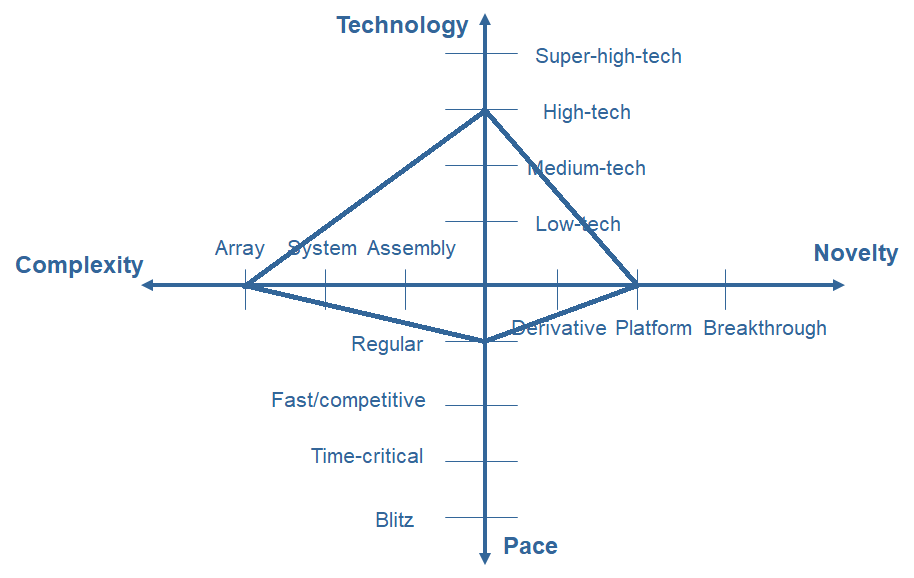
\includegraphics[width=\textwidth]{NationalProgrammeForITNTCP.png}
				\caption{Shows the NTCP Diamond created for the National Programme for IT project}
				\label{fig:NTCPDigram}
			\end{figure}
			\paragraph{Technology}
			{
				I've decided that the technological aspects are High tech this is due to the type of the project as it is a software project therefore will need to use the latests technologies and systems for it to run. also considering that this was launched in the early 2000's we should recognise that although it would probably be a medium tech project today the fact that software projects of this size would not have been though often back then, leads this to require a higher level of technology.
			}
			\paragraph{Novelty}
			{
				A software project of this size and complexity would very much have been the first of it's kind when it was first mentioned however a lot of the techniques and architecture would have been standard and commonplace. According to Taghreed Justinia it was \textquote{Deemed the world’s largest civil IT programme}\cite{Justinia2016}. 
			}
			\paragraph{Pace}
			{
				The National programme for IT was originally launched in 2002 and was scheduled to finish in December 2010 however by 2011 it was still unfinished and was dismantled to salvage services from the project, this shows that it was a very long term project. Also, due to the type of project it was the problem it was required for and the benefits it would provide would not change over time meaning this was not a time sensitive project with the only real limitation being the additional costs of taking more time to develop a product.
			}
			\paragraph{Complexity}
			{
				The main reason why I have labelled this project as very complex is due to the size of the project the original aim was to provide a large number of services as a part of the project. Each of the services would have probably been considered a system on their own however due to the fact all of them have been merged I have labelled the project as a project of Array level complexity.
			}
		}
		\subsection{Is it A Copps}
		{
			Looking at the NTCP Dimond you can see that the only low ranking feature is the time feature with all of the other features being of medium to high ranking. Also the complexity of the project is large but also the scale of the project is large as it covers all of England which is around 50 million people around the time of production\cite{NationalStatistics2018}. The fact that it covers not just one service but multiple services including physical broadband access\cite{Health2002} and software systems. Therefore I would comfortably put it in the realm of Copps projects. 
		}
	}
	\section{Project Life cycle}
	{
		\begin{displaycquote}{Health2002}
			This timeline for phase 0 was from April 2002 to March 2003 and involved preparation tasks such as defining data and communication standards, ensuring that all consultants have PCs, handing out contracts and expanding the NHS IT department to cope with the larger demand which will be placed on it.

			The timeline for phase 1 was from April 2003 to December 2005 and involved providing broadband access to NHS staff. Implementing the national bookings service, 50\% of the National Prescriptions service.

			The timeline for phase 2 is from January 2006 to December 2007 and involved providing Secure access mechanisms for NHS Staff, A full national health service record, A national booking service with all patient appointments, National prescriptions service 100\% implemented, Electronic Patient Records implemented in all NHS trusts, Telemedicine in all GP surgeries. Patient portal via internet, Ambulance Telemonitoring 20\% and radio replacement, National Knowledge service fully established.

			The timeline for phase 3 is from January 2008 to December 2010 and involves implementing Ambulance Telemonitoring to 100\%, Home Telemonitoring to 100\% and a Unified Health Record.
		\end{displaycquote}
		As mentioned in the above quote there are four phases with multiple deliverables. Stretching from the initial mainly planning phase to the delivery phases. The first phase is very much a planning/preparation phase as it focuses on getting the important overall plans ready whilst also preparing the NHS by ensuring NHS Staff have access to PCs and expanding the IT department. Phase 1 and 2 mainly focus on the implementation and contains releases for most of the deliverables for the project. Phase 3 appears to be a finishing/polishing off phase where its focus is on expanding implementation and appears to be a contingency build into the plan.
	}
	\section{User Participation}
	{
		According to Dr Nowlan and Professor Hutton a major reason for the projects failure was due \textquote{clinicians were not taken into account and did not have sufficient say}\cite{Commons2007} this shows the lack of user/customer engagement in the project. It could be argued that this is because of the waterfall approach to product development which only really allows customer input at the beginning of the project whereas agile allows customer input throughout. I will get on to the software development methodologies in \cref{par:softwareDevelopmentMethodology}. The lack of user engagement is probably one of the reasons why the project is considered a failure especially as this is a good example of where user input could be used, as most hospitals and GP surgeries will have systems currently in place and understanding how clinicians use them and how they would like to use them would be a great input for the project. 
	}
	\section{Software Engineering}
	{
		\subsection{Software Development Methodology}
		{
			\label{par:softwareDevelopmentMethodology}
			The National Programme for IT used a waterfall approach for software development\cite{Hoeksma2013}. I would describe this as a major failing in planning and decision making. Generally you would choose a waterfall methodology when your requirements are set in stone and changes to the deliverables of the project are very difficult to implement. In the case of the National Program for IT the requirements were provided at the start however due to the length of time the project covered they changed over the course of the project this also meant that different new technologies emerged which would have made developing the project easier. Also, although some parts of the programme was built on physical infrastructure this meant that some of the deliverables were unable to be changed the majority of the software would be changes easily as is the way with software products. It would have also made more sense to build the programme on top of the internet instead of using their own network as it would have been cheaper and reduce/remove the need for the external contracts and make it more suitable for an agile approach which tends to be cheaper and provide deliverables earlier and allow for more customer input. Hoeksma also goes on to say that \textquote{NHS England recently commissioned a replacement for the NHS “spine,” the data backbone built using the waterfall method. An agile developer quickly delivered a potential replacement for a tenth of the cost of the earlier system.}\cite{Hoeksma2013} which shows how much time and money could have been saved by using an agile methodology when implementing this project.

			One of the failings to use agile software development methodologies may have been down to the top down approach to the development of the systems as traditional engineering projects tend to be more successful with waterfall development therefore the government planners may not have been fully familiar with software systems project planning.

			Some more benefits to using an agile approach would be to develop the project on a smaller scale in terms of developing the system for one hospital/trust to ensure that the system is working well and ready for deployment before deploying to the rest of the country however this could also be implemented with waterfall if there are any problems during the initial deployment it makes it harder and more costly to change the system and fix the problems.
		}
		\subsection{Using open source software}
		{
			Making some sort of use of opens source software could have been an alternative option as it could make the development process easier although there is some open source software which cannot be sold as a part of another product this can be avoided by developing the software within the NHS meaning that the NHS would have to start a software development program and then develop the project in house this would allow for all forms of open source software to be used. This form of development would be more difficult and costly but would also allow for the project to be treated like a product instead of a project and get updates and support over the life of the product.\textquote{Whilst using open source and open standards can solve some of the problems in the delivery of information systems for the NHS}\cite{chelsom2011open}.
		}
	}
	\section{Project Organisation}
	{
		\begin{figure}
			\centering
			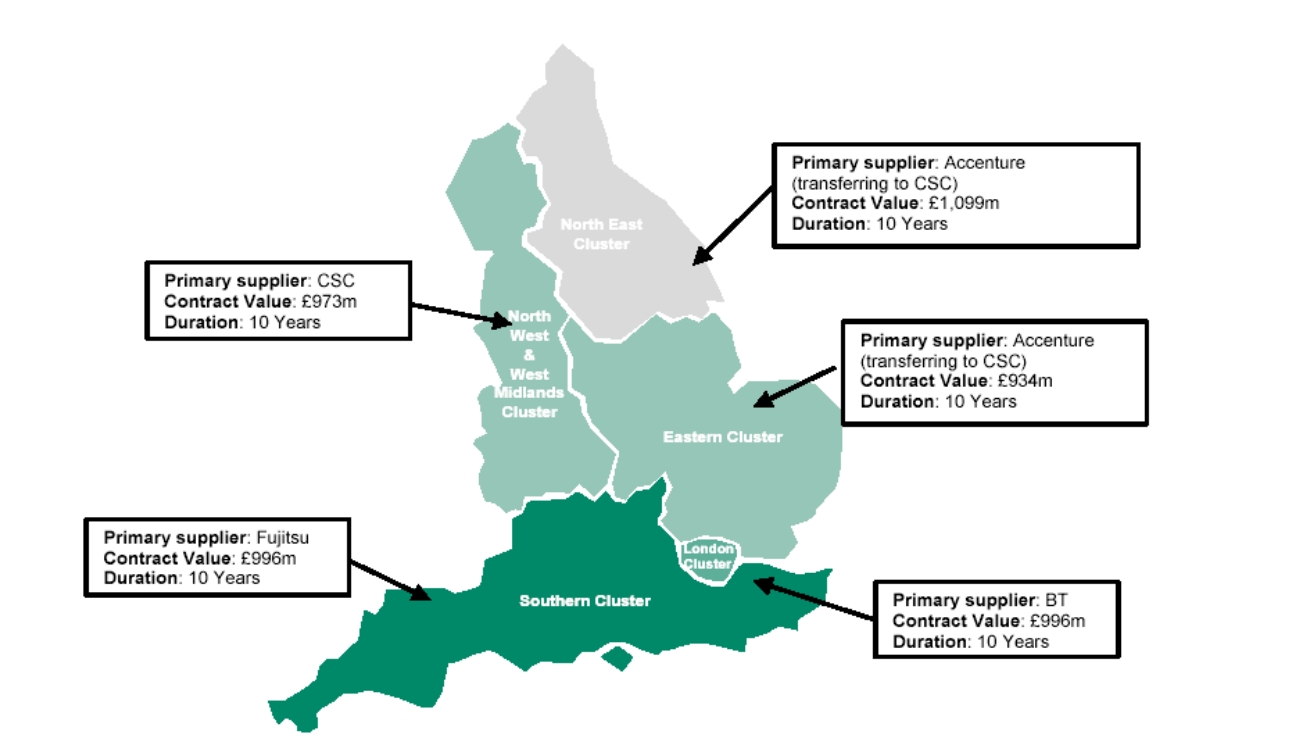
\includegraphics[width=\textwidth]{NPfITClusterContracts}
			\caption{Shows a breakdown of the clusters for the UK and the contractors assigned to the clusters\cite{Campion-Awwad2014}}
			\label{fig:NPfITClusterContracts}
		\end{figure}
		\begin{figure}
			\centering
			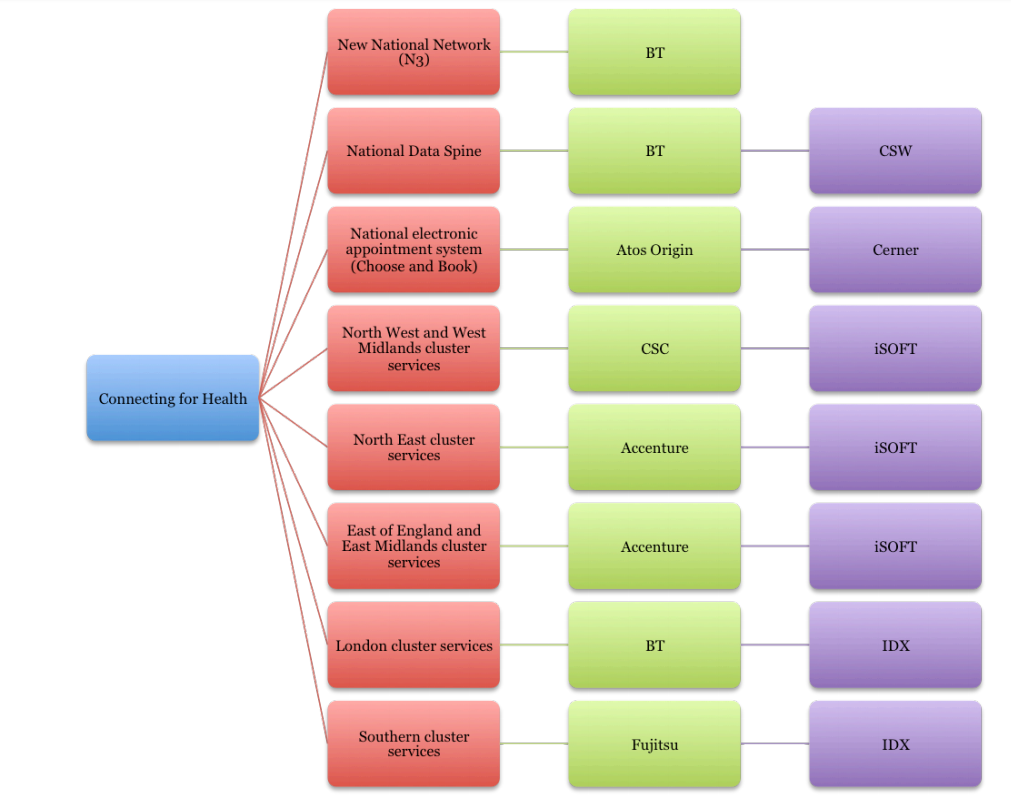
\includegraphics[width=\textwidth]{NPfITContractBreakdown}
			\caption{Shows a breakdown of the which contractor implemented which services and the software subcontractors used\cite{Campion-Awwad2014}}
			\label{fig:NPfITContractBreakdown}
		\end{figure}
		As you can see from \Cref{fig:NPfITServicesOutline} many of the services provided were broken up to be implemented by multiple contractors which matches a Project Based Organisation Structure. However it appears that rather than breaking down the project into multiple separate services they broke it down by region which is a major failing from a project management point of view. According to \cref{fig:NPfITContractBreakdown} the cluster services are implemented by 4 different contractors and 2 different software contractors meaning that each of the software contractors would be implementing broadly speaking the same system with the same functionality completely independently. Considering how easily reproducible software is this is a major failing. As it would have been far more efficient for one software contractor to be used for implementing the cluster services. Also some of the services were delivered before the project was being dismantled\cite{Charette2011} this then begs the question if these services were delivered why not make them completely orthogonal and attempt the project using a divide and conquer approach. There would be many benefits to this such as being able to complete the smaller project quicker and more efficiently. Being able to train users at a slower pace as the new systems would be implemented linearly. The ability to manage each service individually meaning less money is wasted and tighter controls on deadlines. Also the benefit of if one of the projects fail the others should not be affected.
	}
	\section{Integration with Current Systems}
	{
		One of the requirements for the project was for the local trusts to implement their own system to transfer the current patient information to the new National Programme for IT system. The National Programme for IT Implementation Guide\cite{HealthImplementationGuidanceteam2007} gives an overview of how the systems should be implemented and suggests that software should be developed using national standards.
	}
	\section{Project Success}
	{
		Most people would categorically say no this project was not a success as it was over budget and never completed. although if you consider the value for money aspect of the project the costs are around £9.8 billion and the benefits are around £10.7 billion\cite{Campion-Awwad2014} which shows that there is still some benefit from the project although this cannot be used as an example of success as it still failed to meet many of the project goals and deadline and cost more than expected. You also need to look at the fact that this system will probably have to be implemented again at some point because the initial ideas are good and provide many benefits to the NHS and public it appears just the execution was flawed. Therefore I believe that the project should be considered a failure.
	}
	\section{Conclusion}
	{
		In conclusion the National Programme for IT is a very useful idea based around the centralising of IT systems and patient information to allow the different parts of the NHS to communicate and work together more efficiently. The project is complex and technologically demanding and while something of this size and span had not been attempted before there are similar systems in place on a smaller scale, the project is not time sensitive and it is a Copps project. The project plan was for a 8 year project from April 2002 to December 2010 although it overran to September 2011 at which point it was dismantled to salvage some services. The clinicians and other stakeholders who were set to use the services were not consulted enough before and during project development. The software development methodologies were very poor and leave a lot of room for improvement also the development of software engineering from the 2000's to now mean that there are far better practices and planning structures to support the development of large systems. Using open source software would have possibly given an advantage to the developers while also saving time and money although using an in house team of developers would be costly to set up although would allow for a better system overall to be produced with better maintenance. Project organisation could also be vastly improved an attempt was made to split up the project into manageable chunks however it was done incorrectly by splitting the problem into geographical areas rather than by the required services. The splitting of services by geographical area made sense for the physical infrastructure needs however for the services development it would have been far more useful to spit it by services or separate the infrastructure from the software development contracts. The integration with current systems went well from my research I couldn't find any problems with this however this could be down to a lack of deployed systems. The project overall cannot be considered a success however as identified in this report there were many failing and much room for improvement therefore the project itself is not fundamentally flawed it simply needs to be executed with better planning.
	}
	
	
	\newpage
	
	\printbibliography[heading=bibintoc,title=References]
\end{document}
